\documentclass[letter,11pt]{beamer}

%spell related
\usepackage[spanish,es-nodecimaldot]{babel}
\usepackage[utf8]{inputenc}

%fonts related
\usepackage{helvet}
\renewcommand{\familydefault}{\sfdefault}
\usepackage{textcomp}

%graphics related
\usepackage{adjustbox}
\usepackage{graphicx}
\usepackage{pstricks}

\usepackage{graphicx}
\usepackage{array}

\usetheme{Pittsburgh}
\setbeamerfont{frametitle}{size=\normalsize}

\title{\textbf{LABORATORIO DE FÍSICA BÁSICA I - GRÁFICOS Y ECUACIONES}}
\subtitle{\textbf{Relación lineal}}
\author{\small{Caballero Burgoa, Carlos Eduardo}}
\date{\tiny{Noviembre 2020}}

\begin{document}

\begin{frame}
\titlepage
\end{frame}

\section{Relación lineal}

\subsection{Serie 1}
\begin{frame}
\frametitle{Serie 1}
    \begin{figure}[!h]
        \centering
        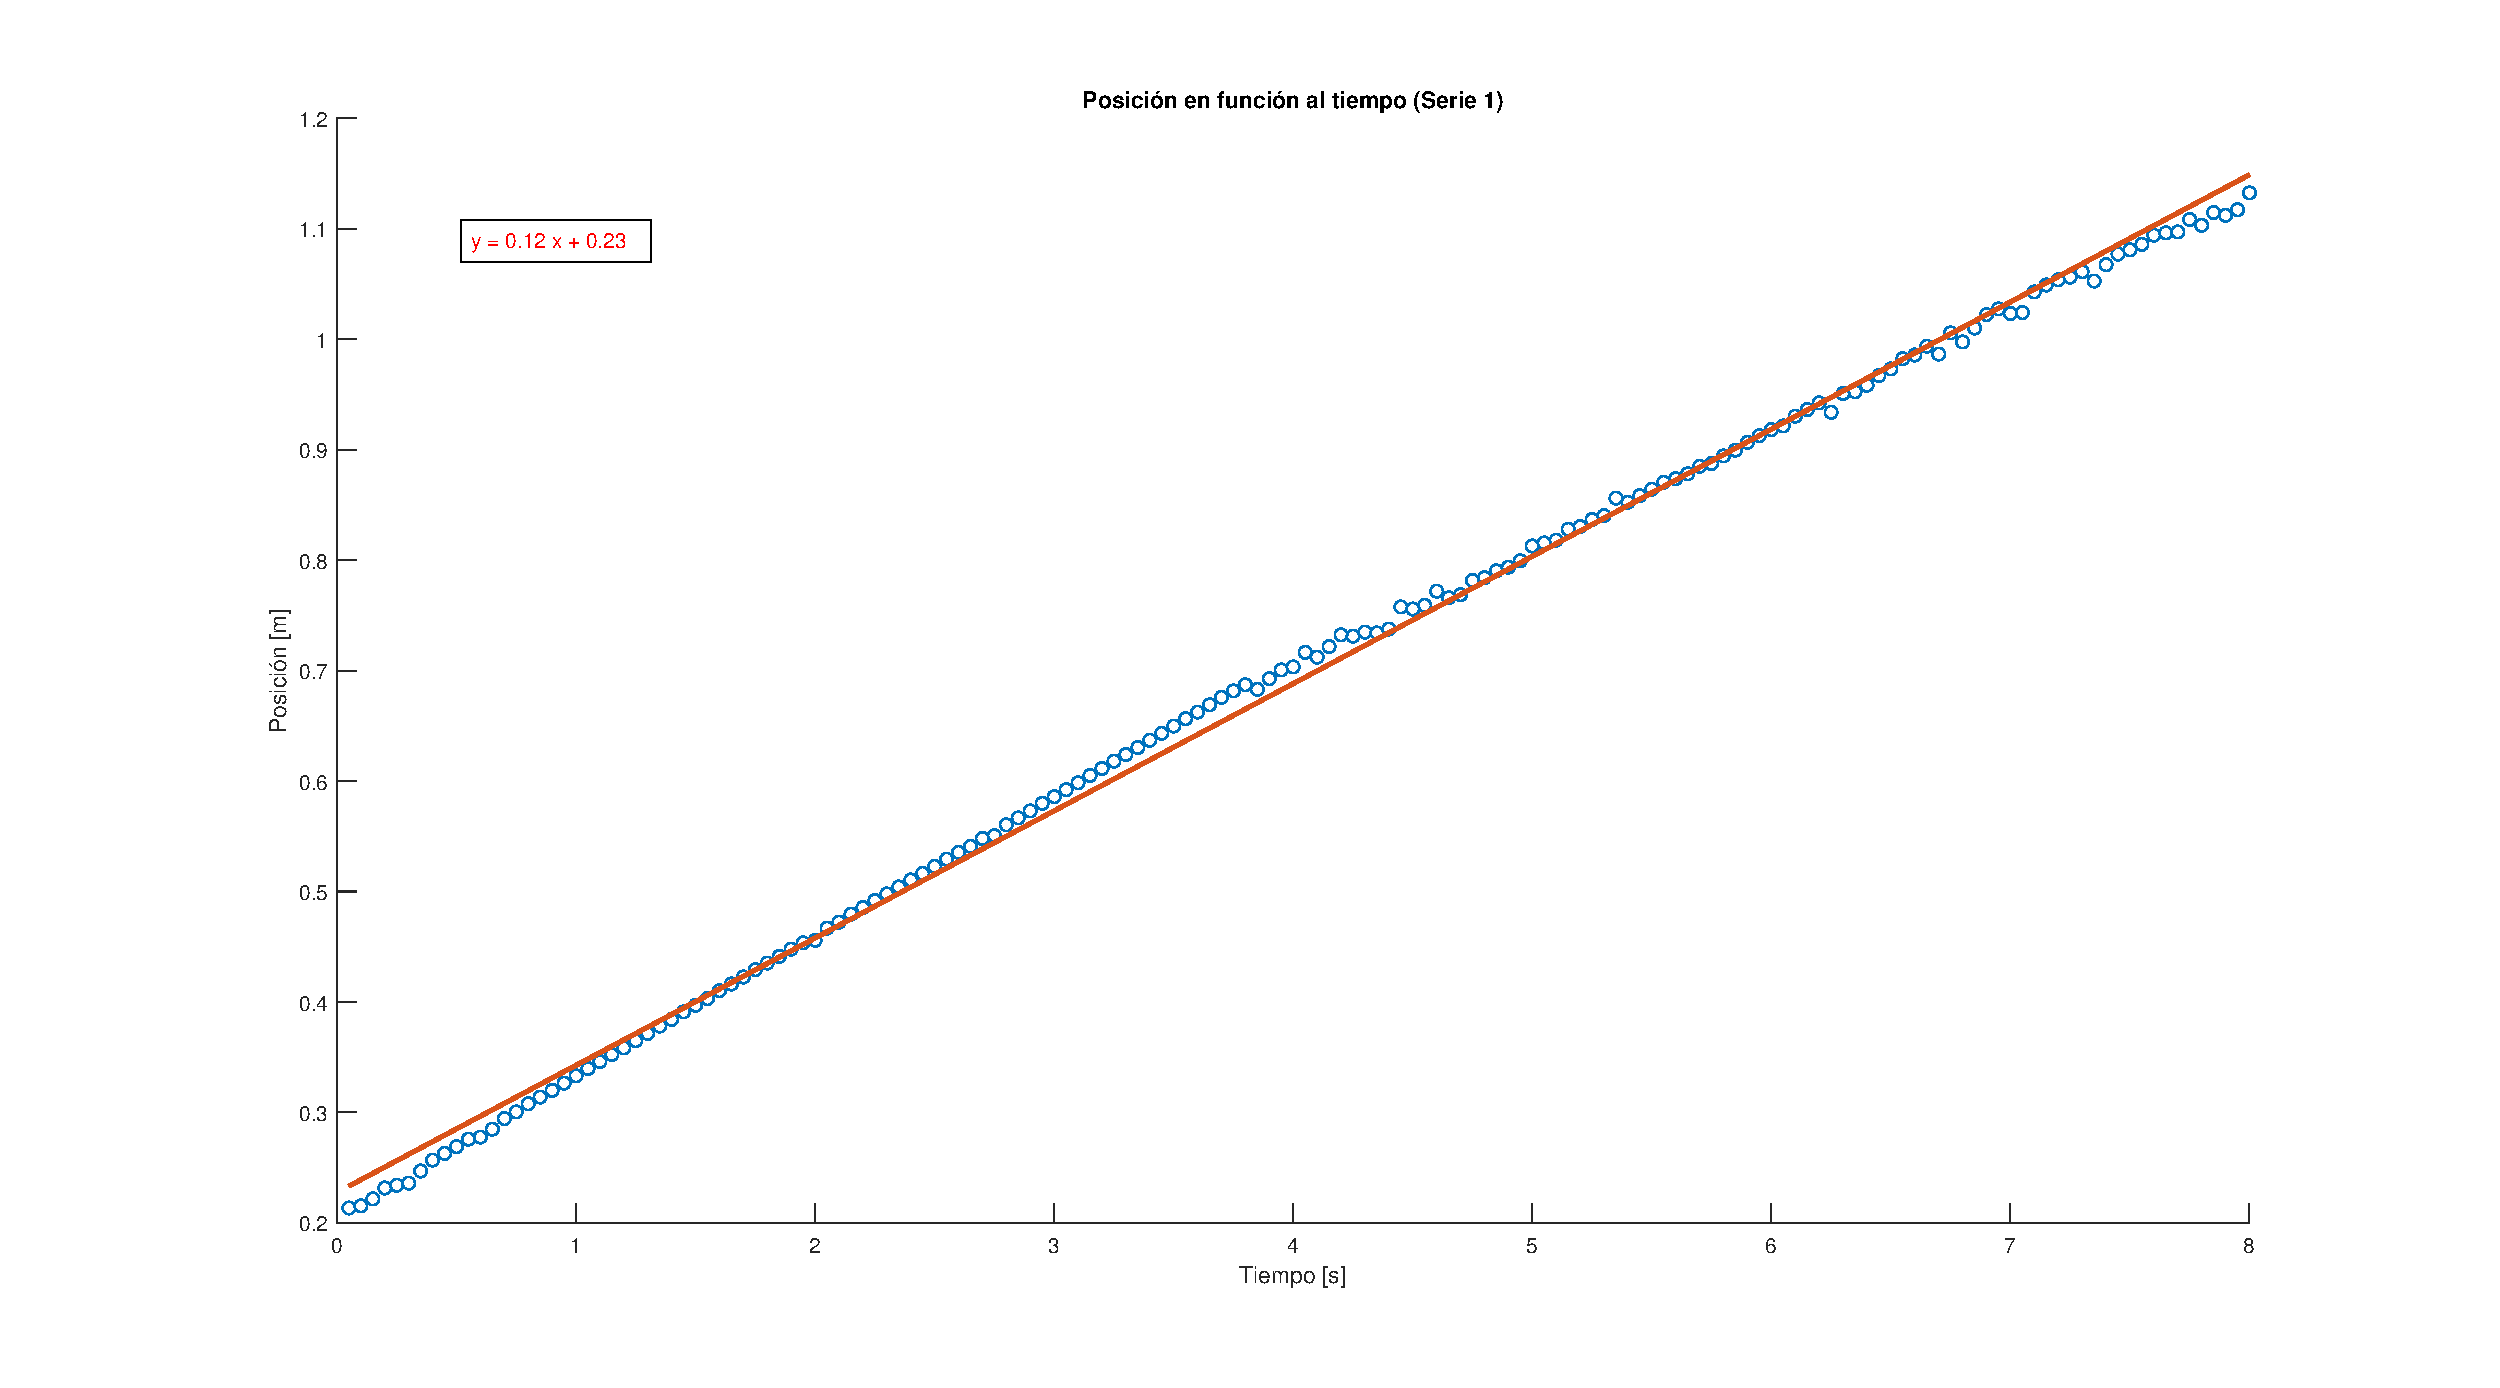
\includegraphics[scale=0.28]{eps/2_5.1.eps}
    \end{figure}
\end{frame}

\subsection{Serie 2}
\begin{frame}
\frametitle{Serie 2}
    \begin{figure}[!h]
        \centering
        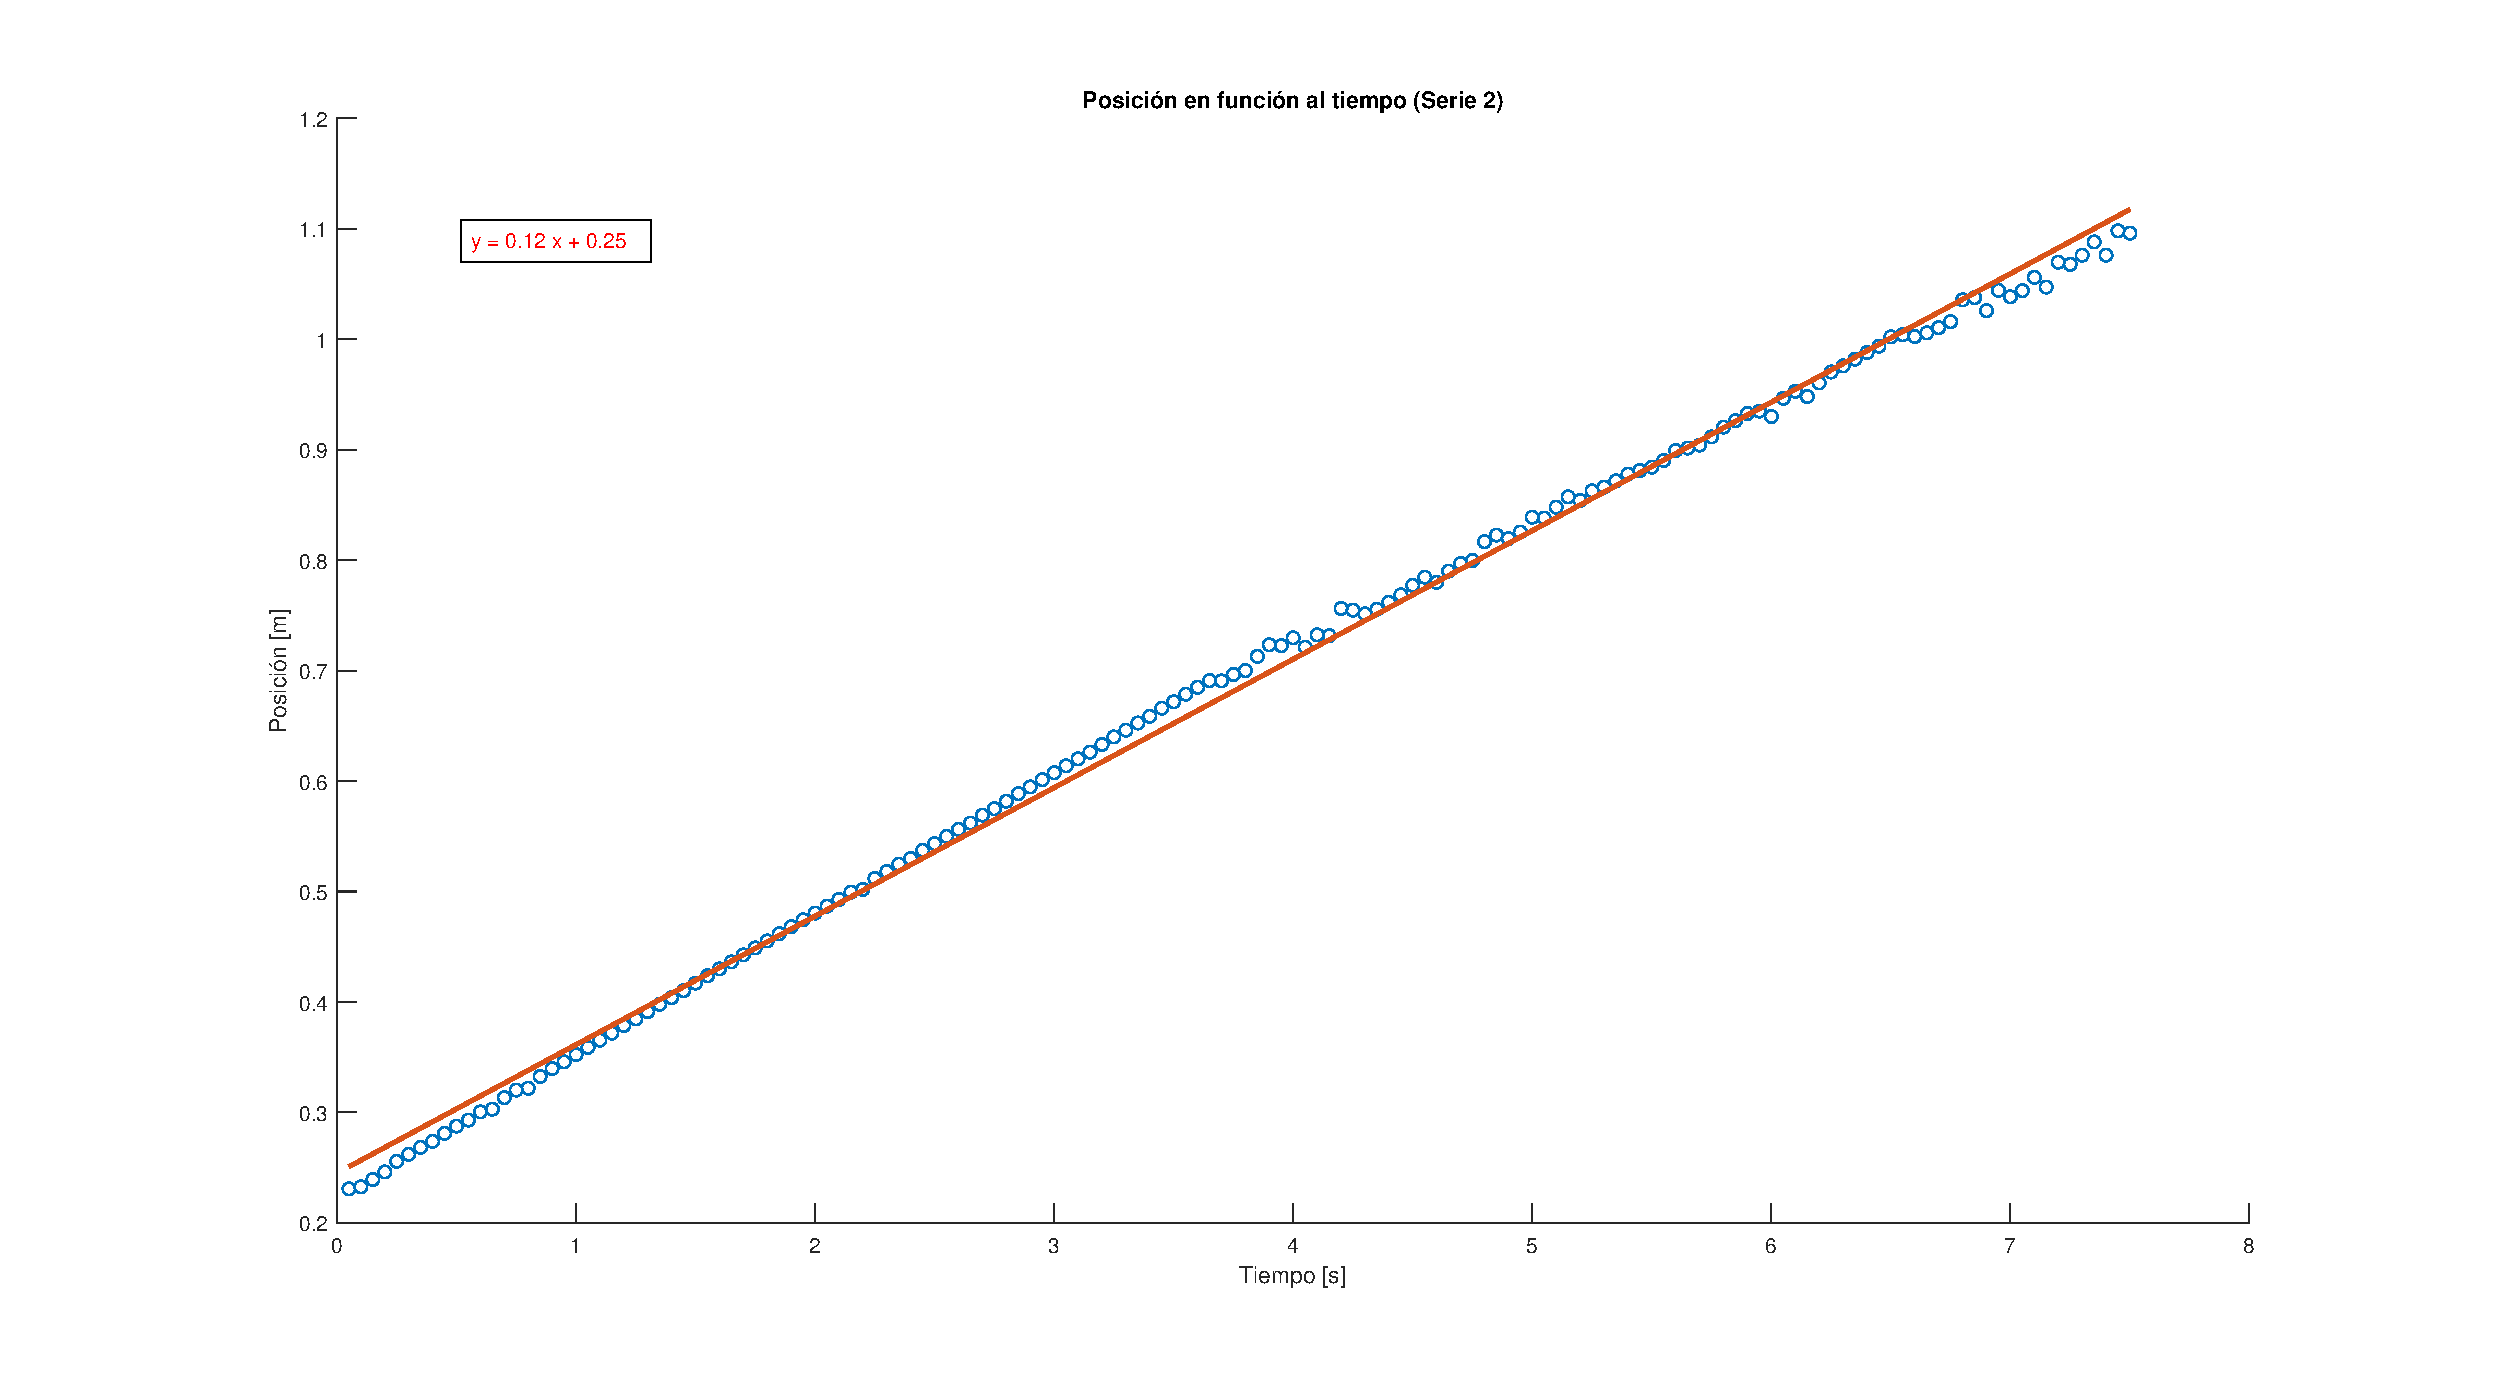
\includegraphics[scale=0.28]{eps/2_5.2.eps}
    \end{figure}
\end{frame}

\subsection{Serie 3}
\begin{frame}
\frametitle{Serie 3}
    \begin{figure}[!h]
        \centering
        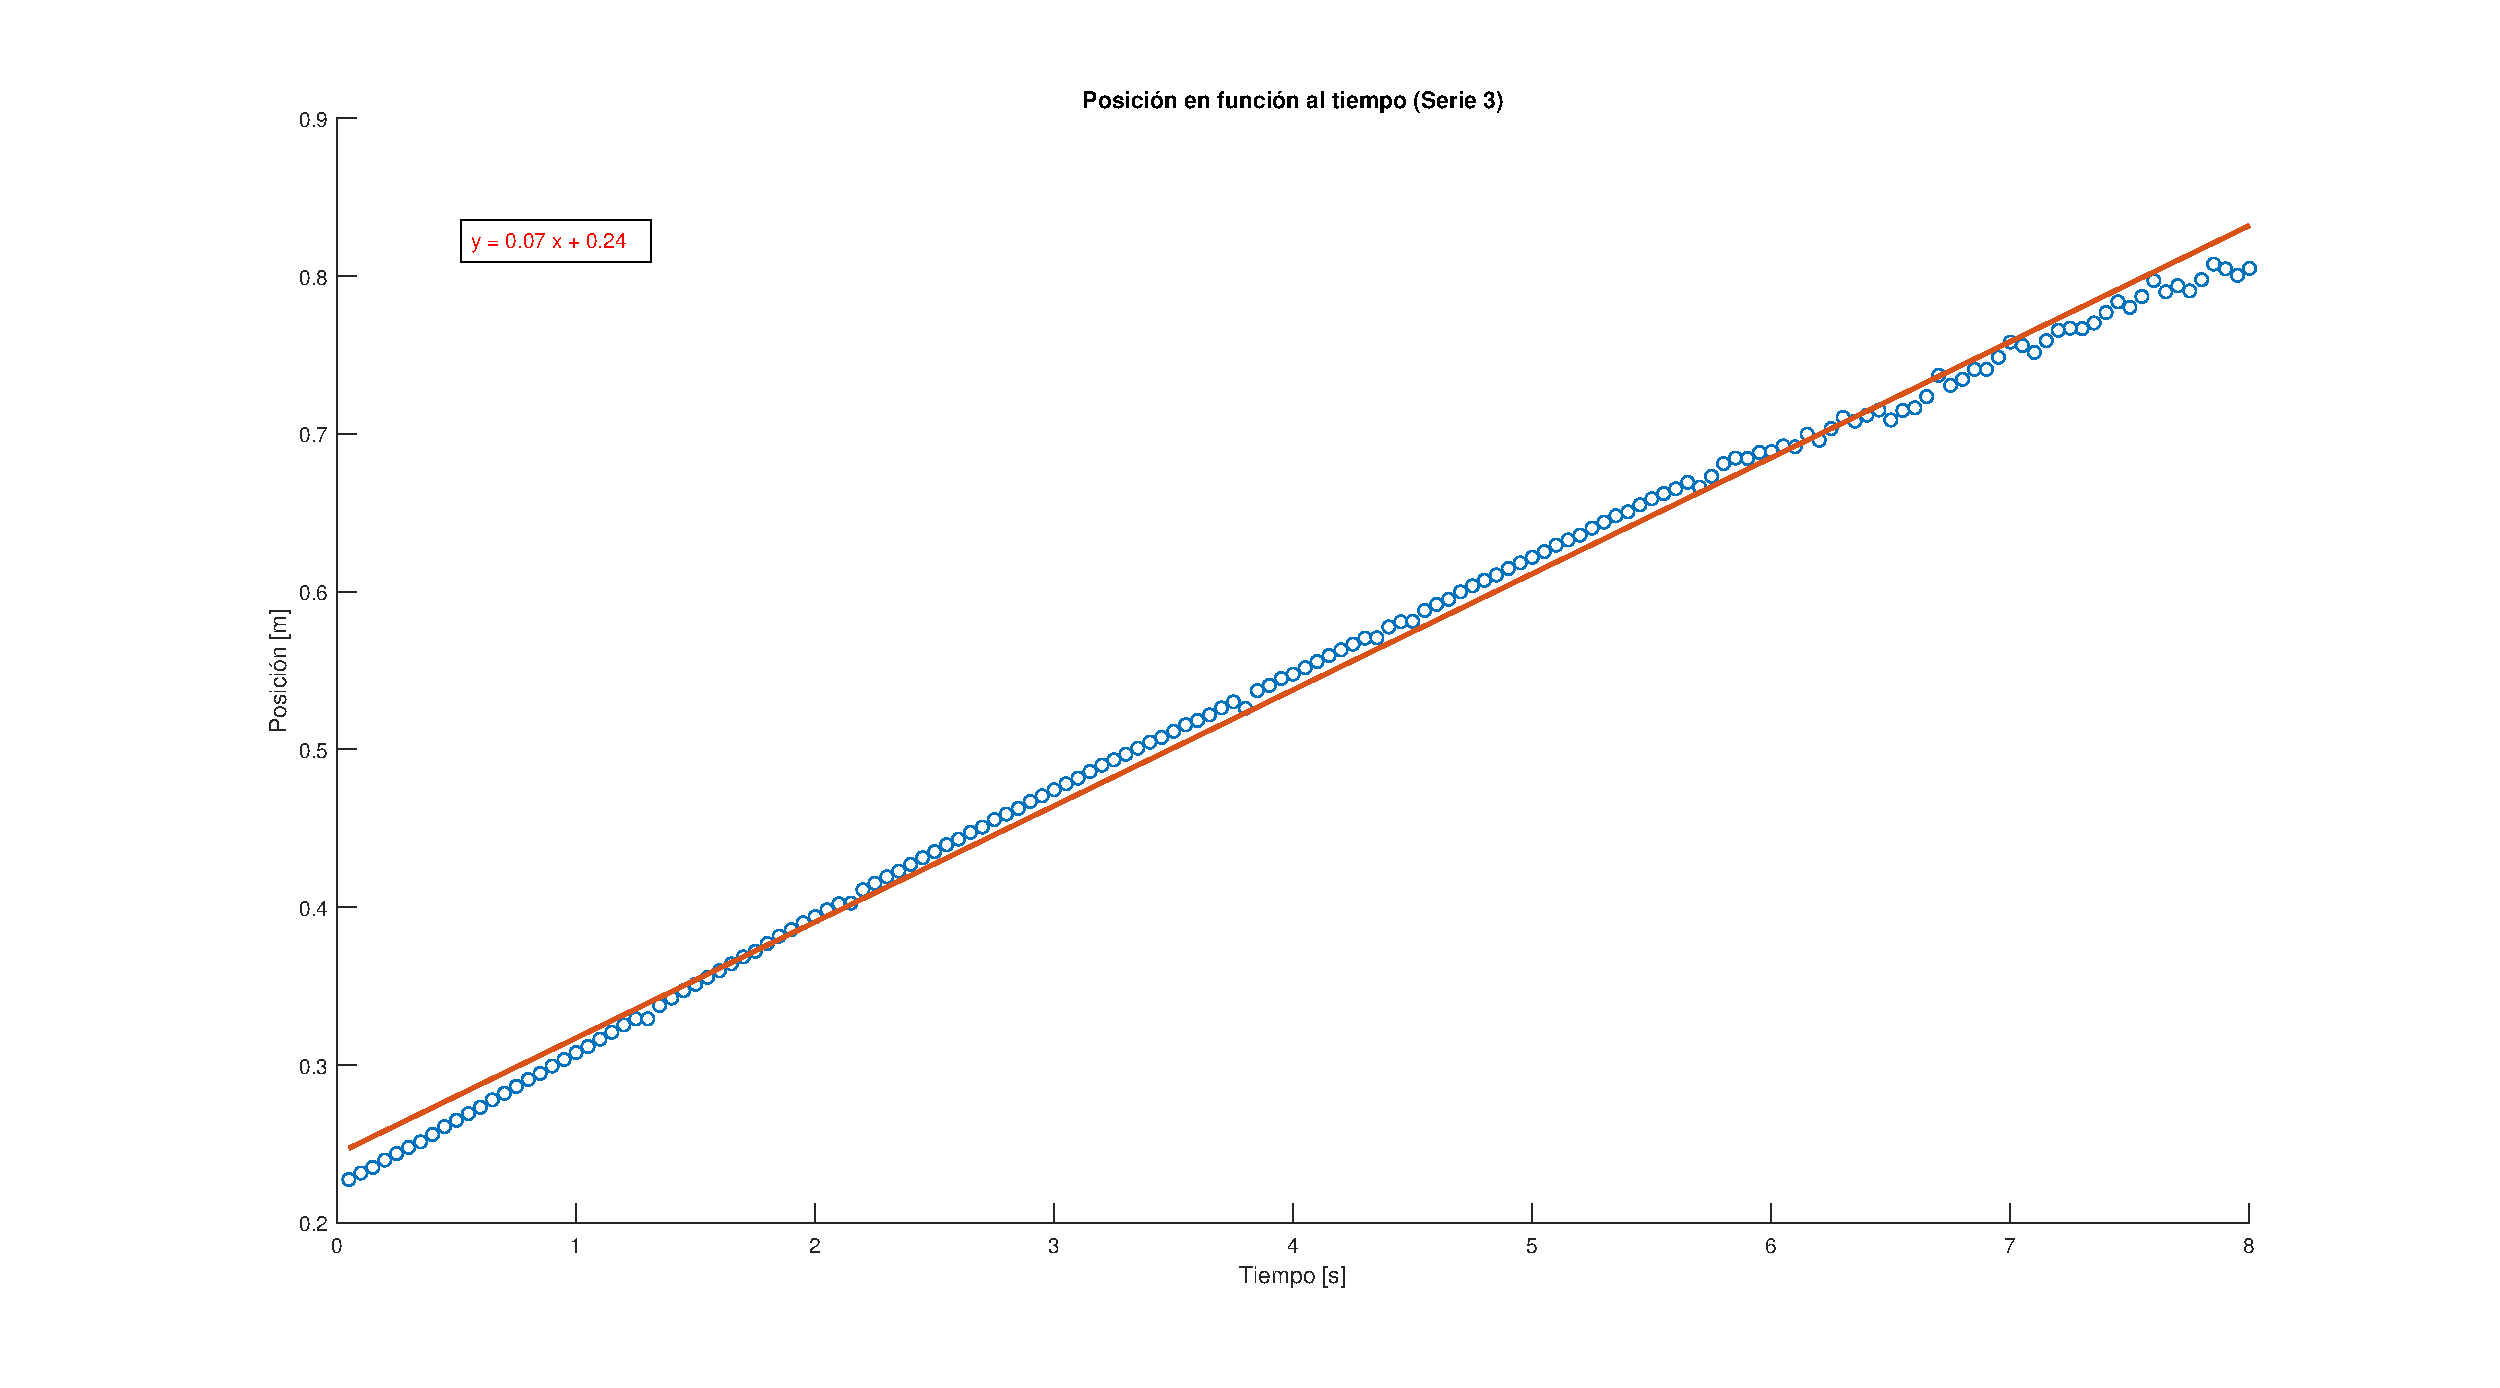
\includegraphics[scale=0.28]{eps/2_5.3.eps}
    \end{figure}
\end{frame}

\end{document}

